\begin{titlepage}
\centering
\vspace*{3.5cm}
{\Huge\bfseries Cálculo de Malliavin\par}
\vspace{1cm}
{\Large de los procesos estocásticos y la integral de Itô\\ al estado del arte\par}
\vspace{1.2cm}
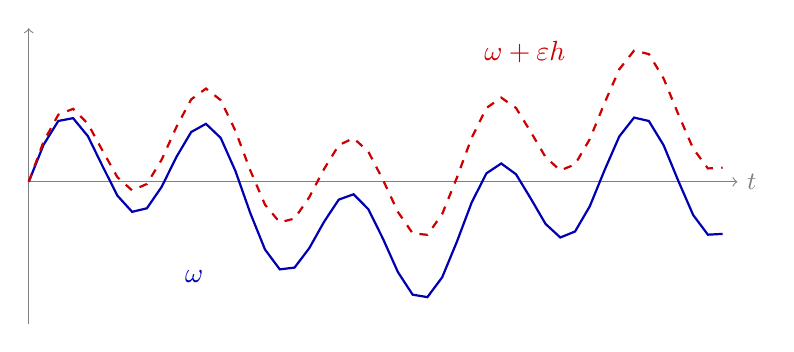
\begin{tikzpicture}[x=0.75cm,y=0.75cm]
  \draw[->,gray] (0,0) -- (12,0) node[right] {\small $t$};
  \draw[->,gray] (0,-2.4) -- (0,2.6);
  \pgfmathsetseed{7}
  \draw[blue!70!black,thick] (0,0)
    \foreach \x in {1,...,47} { -- (\x/4, {0.9*sin(\x*37) + 0.6*sin(\x*11) - 0.03*\x + 0.04*(\x-20)*(\x>20)}) };
  \draw[red!80!black,thick,dashed] (0,0)
    \foreach \x in {1,...,47} { -- (\x/4, {0.9*sin(\x*37) + 0.6*sin(\x*11) - 0.03*\x + 0.04*(\x-20)*(\x>20) + 0.025*\x + 0.4*sin(\x*4)}) };
  \node[blue!70!black] at (2.8,-1.6) {$\omega$};
  \node[red!80!black] at (8.4,2.2) {$\omega+\varepsilon h$};
\end{tikzpicture}
\vspace{1.5cm}

{\large Una guía con demostraciones\par}
\vfill
{\large Noviembre de 2026\par}
\end{titlepage}
